\documentclass[12pt,a4paper]{article}

\usepackage[a4paper, top = 2cm, bottom = 2cm, left = 1.5cm, right = 1.5cm]{geometry}
\usepackage[dvipsnames]{xcolor} % Colors

\usepackage{standalone}

\usepackage{setspace}
\usepackage{graphicx}
\usepackage{amsfonts}
\usepackage{amsmath}
\usepackage{tikz}
\usepackage{pdfpages}
\usepackage{epigraph}
\usepackage{csquotes}

% Bibliography
\usepackage{xcolor}
\usepackage{hyperref}
\hypersetup{
    colorlinks=true,
    citecolor=MidnightBlue,
		linkcolor=MidnightBlue,
    pdfpagemode=FullScreen,
    }

\usepackage{natbib}
\usepackage[noabbrev]{cleveref}
\setcitestyle{authoryear,open={(},close={)}}
\bibliographystyle{plainnat}

\usepackage{subfiles}

\setlength\parindent{0pt}
\spacing{1.2}

\begin{document}

\begin{center}
       \vspace*{1cm}
       \huge\textbf{Problemset 1} \\
       \vspace{0.4cm}
       \large \textbf{Public Finance in Macroeconomics} \\
       \vspace{0.5cm}
        \large Handed in by the \textcolor{orange}{\textbf{Heterogeneous Geeks}} \\ 
        
        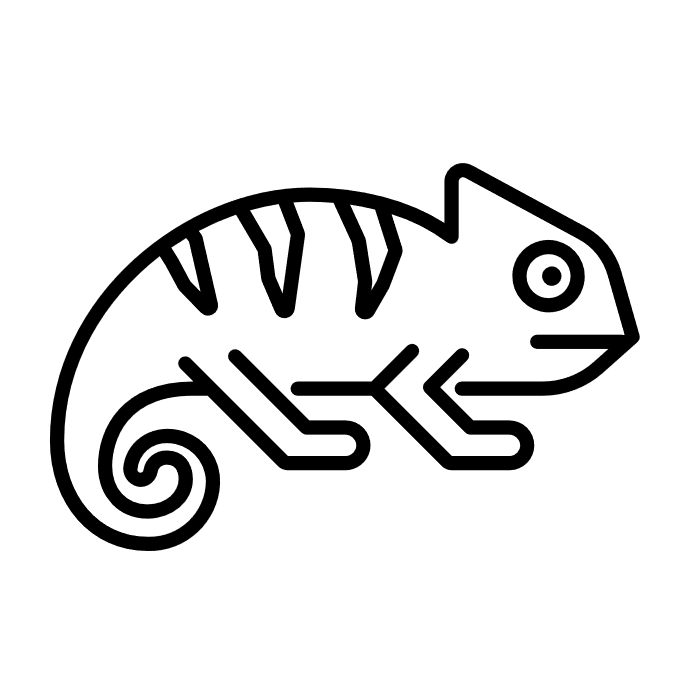
\includegraphics[scale=0.1]{geek.png} \\ 
        \vspace{0.3cm}
        a.k.a. Vivien Voigt, Thong Nguyen, \\Davide Difino \& Celina Proffen \\
       \vspace{1.5cm}
       \vfill
       
       % I also thought of adding some cool superheroe image her, but I didn't find one - feel free to delete the gecko if you don't like it/ find it appropriate! ;)
       
        Problem set in the context of Prof. Ludwig's course: \\
        \textbf{Public Finance in Macroeconomics: Heterogenous Agent Models}\\
        at the Graduate School of Economics Finance and Management
       \vspace{0.8cm}
   \end{center}

\section*{Problem 1}

\begin{itemize}
  \item The marginal utility are given by:

      $$ u'(c) = (1-\sigma) \cdot \frac{1}{1-\sigma} c^{1-\sigma - 1} = c^{-\sigma} $$

    and

      $$ u''(c) = -\sigma c^{-\sigma -1}$$

    Therefore the coefficient of relative risk aversion is:

      $$ -\frac{u''(c)}{u'(c)}\cdot c = \frac{\sigma c^{-\sigma -1}}{c^{-\sigma}} \cdot = \sigma $$

    The coefficient in the CRRA utility measures the risk aversion of the individual.

  \item Adding a constant value is a monotonic trasformation therefore the ordinal property of the utility index does \textbf{not} change and the utility function still represent the same underlying preferences.

  \item The limit is:

    $$ \lim_{\sigma \to 0} \frac{c^{1-\sigma} - 1}{1-\sigma} = \frac{0}{0} \quad \forall t, s^t.$$

  Therefore the de l'Hopital Theorem apply. That is:

    $$\lim_{\sigma \to 1} \frac{c^{1-\sigma} - 1}{1-\sigma} = \lim_{\sigma \to 1} \frac{\partial [c^{1-\sigma} - 1]}{\partial \sigma} \frac{\partial \sigma}{\partial 1-\sigma} = \lim_{\sigma \to 1} \frac{- c^{1-\sigma} \log c}{-1} = \log c.$$

  \item The consumption growth pattern is such that

    $$  \bar{c}_0 = (1 + g) \cdot c_0 \qquad \bar{c}_1 = (1 + g) \cdot \bar{c}_1 $$;

  therefore

    $$  u(\bar{c}) = \frac{\bar{c}_0^{1 - \sigma}}{1 - \sigma} + \beta \frac{\bar{c}_1^{1 - \sigma}}{1 - \sigma} = \frac{[(1 + g) \cdot c_0]^{1-\sigma}}{1-\sigma} + \beta \frac{[(1 + g) \cdot c_1]^{1-\sigma}}{1-\sigma}. $$

  Collecting yields

  $$  u(\bar{c}) = \frac{(1 + g)^{1-\sigma} \cdot c_0^{1-\sigma}}{1-\sigma} + \beta \frac{(1 + g)^{1-\sigma} \cdot c_1^{1-\sigma}}{1-\sigma} = (1 + g)^{1-\sigma} \left[  \frac{c_0^{1 - \sigma}}{1 - \sigma} + \beta \frac{c_1^{1 - \sigma}}{1 - \sigma} \right] = (1 + g)^{1-\sigma} u(c).$$
  
  This type of preferences are called additively separable. 

  \item  Assume $u(\bar{c}) = (1 + g)^{1-\sigma} u(c)$
    \begin{align*}
      \Rightarrow & \quad \frac{[(1 + g) \cdot c_0]^{1-\sigma} - 1}{1-\sigma} + \beta \frac{[(1 + g) \cdot c_1]^{1-\sigma} - 1}{1-\sigma} = (1+g)^{1 - \sigma} \cdot \left( \frac{c_0^{1-\sigma} - 1}{1-\sigma} + \beta \frac{c_1^{1-\sigma} - 1}{1-\sigma} \right) \\
      & \\
      \Rightarrow & \quad [(1 + g) \cdot c_0]^{1-\sigma} - 1 + \beta [(1 + g) \cdot c_1]^{1-\sigma} - 1 = (1+g)^{1 - \sigma} \cdot \left( c_0^{1-\sigma} - 1 + \beta c_1^{1-\sigma} - 1 \right) \\
      & \\
      \Rightarrow & \quad [(1 + g) \cdot c_0]^{1-\sigma} + \beta [(1 + g) \cdot c_1]^{1-\sigma} - 2 = [(1 + g) \cdot c_0]^{1 - \sigma} + \beta [(1 + g) \cdot c_1]^{1-\sigma}- 2 \cdot (1 + g)^{1 - \sigma}.
    \end{align*}
That is, $ 2 = 2 \cdot (1 + g)^{1 - \sigma} \quad \Rightarrow \quad (1 + g)^{1 - \sigma} = 0 \quad \Rightarrow\Leftarrow \quad \forall g \neq 0 \qquad QED$

\end{itemize}

\section*{Problem 2}

\begin{itemize}

  \item The social planner problem is:

    \begin{align*}
      & \max_{\{ c_t^1, c_t^2 \}^{\infty}_{t = 0}} \sum^\infty_{t=0} \beta^t [\alpha \ln c_t^1 + (1-\alpha) \ln c_t^2] \\
      & \text{s.t.} \\
      & c_t^i \geq 0 \qquad \forall i, t \\
      & c^1_t + c^2_t = 2 \quad \forall t.
    \end{align*}

    \textbf{Step 1}: The Lagrangian (with scaled multiplier $\frac{\mu_t}{2}$) is

    $$
      \mathbb{L} = \sum^\infty_{t=0} \beta^t [\alpha \ln c_t^1 + (1-\alpha) \ln c_t^2] + \frac{\mu_t}{2} [2 - c_t^1 - c_t^2],
    $$

    whose FOCs are:

    \begin{align*}
      & \frac{\alpha \beta^t}{c_t^1} - \frac{\mu_t}{2} = 0 & \Rightarrow & \qquad \frac{\mu_t}{2} = \frac{\alpha \beta^t  }{c_t^1} \\
      & \frac{(1 - \alpha) \beta^t}{c_t^2} - \frac{\mu_t}{2} = 0 & \Rightarrow & \qquad \frac{\mu_t}{2} = \frac{(1 - \alpha) \beta^t}{c_t^2} \\
    \end{align*}.

    It follows that

    $$
    \frac{(1 - \alpha)\beta^t}{c_t^2} = \frac{\alpha \beta^t  }{c_t^1} \qquad \Rightarrow \qquad \frac{c_t^1}{c_t^2} = \frac{\alpha}{1 - \alpha}.
    $$

    Substituting the budget constraint yields

    $$
      c_1^t + c_t^2 = 2 \quad \Rightarrow \quad c_1^t + \frac{1 - \alpha}{\alpha} c_t^1 = 2 \quad \Rightarrow \quad \left(1 + \frac{1 - \alpha}{\alpha} \right) \cdot c_t^1 = 2 \quad \Rightarrow \quad c_t^1 (\alpha) = 2 \alpha
    $$

    thus $c_t^2 (\alpha) = 2(1-\alpha)$.

    \textbf{Step 2}: The transfer function, that is the amount of resources that agent $i$ must receive (or give) in order to be able to afford the planner's allocation given $\alpha$ and her resources $y^i_t$ in period $t$ is:

      $$
      t^i(\alpha) = \sum_{t} \beta^t \left( c_t^i(\alpha)- y_t^i \right)
      $$

    that is

    \begin{align*}
      & t^1(\alpha) = \sum_{t} 2 \beta^t \alpha - \sum_{t} \beta^t  y_t^1 \\
      & t^2(\alpha) = \sum_{t} 2 \beta^t (1 - \alpha) - \sum_{t} \beta^t y_t^2.
    \end{align*}

    Notice that

    \begin{align*}
      & \sum_{t} \beta^t  y_t^1 = \cdot (0 + 2\beta^2 + 0 + 2\beta^4 + \ldots) = 2 \cdot \sum \beta^{2t}  \\
      & \sum_{t} \beta^t  y_t^2 = \cdot (2\beta + 0 + 2\beta^3 + \ldots) = 2 \cdot \sum \beta^{2t - 1} = 2 \beta \cdot \sum \beta^2t,
    \end{align*}

  therefore

  \begin{align*}
    & t^1(\alpha) = 2\alpha \cdot \sum_{t} \beta^t - 2 \cdot \sum_{t} \beta^{2t} =  \frac{2\alpha}{1 - \beta} - \frac{2}{1 - \beta^2}\\
    & t^2(\alpha) = 2(1 - \alpha) \cdot \sum_{t} \beta^t - 2\beta \cdot \sum_{t} \beta^{2t} = \frac{2 (1 - \alpha)}{1 - \beta} - \frac{2 \beta}{1 - \beta^2}.
  \end{align*}

  \textbf{Step 3}: in a competitive equilibrium there are no transfer, thus

  \begin{align*}
    & t^1(\alpha) = 0 \quad \Rightarrow \quad \frac{2\alpha}{1 - \beta} = \frac{2}{1 - \beta^2} \quad \Rightarrow \quad \alpha = \frac{1 - \beta}{1 - \beta^2} = \frac{1 - \beta}{(1 - \beta)\cdot(1 + \beta)} = \frac{1}{1 - \beta}  \\
    & t^2(\alpha) = 0 \quad \Rightarrow \quad \frac{2 (1 - \alpha)}{1 - \beta} = \frac{2 \beta}{1 - \beta^2}  \quad \Rightarrow \quad 1 - \alpha = \frac{\beta(1 - \beta)}{1 - \beta^2} = \frac{\beta}{1 - \beta}.
  \end{align*}

  The competitive equilibrium is given by

  \begin{align*}
    & c_t^{1*} = \frac{2}{1+\beta} \\
    & c_t^{2*} = \frac{2\beta}{1+\beta}
  \end{align*}

  \item The tree for both agent (since the states of the world tie both income):

  \begin{figure}[h!]
    \centering
    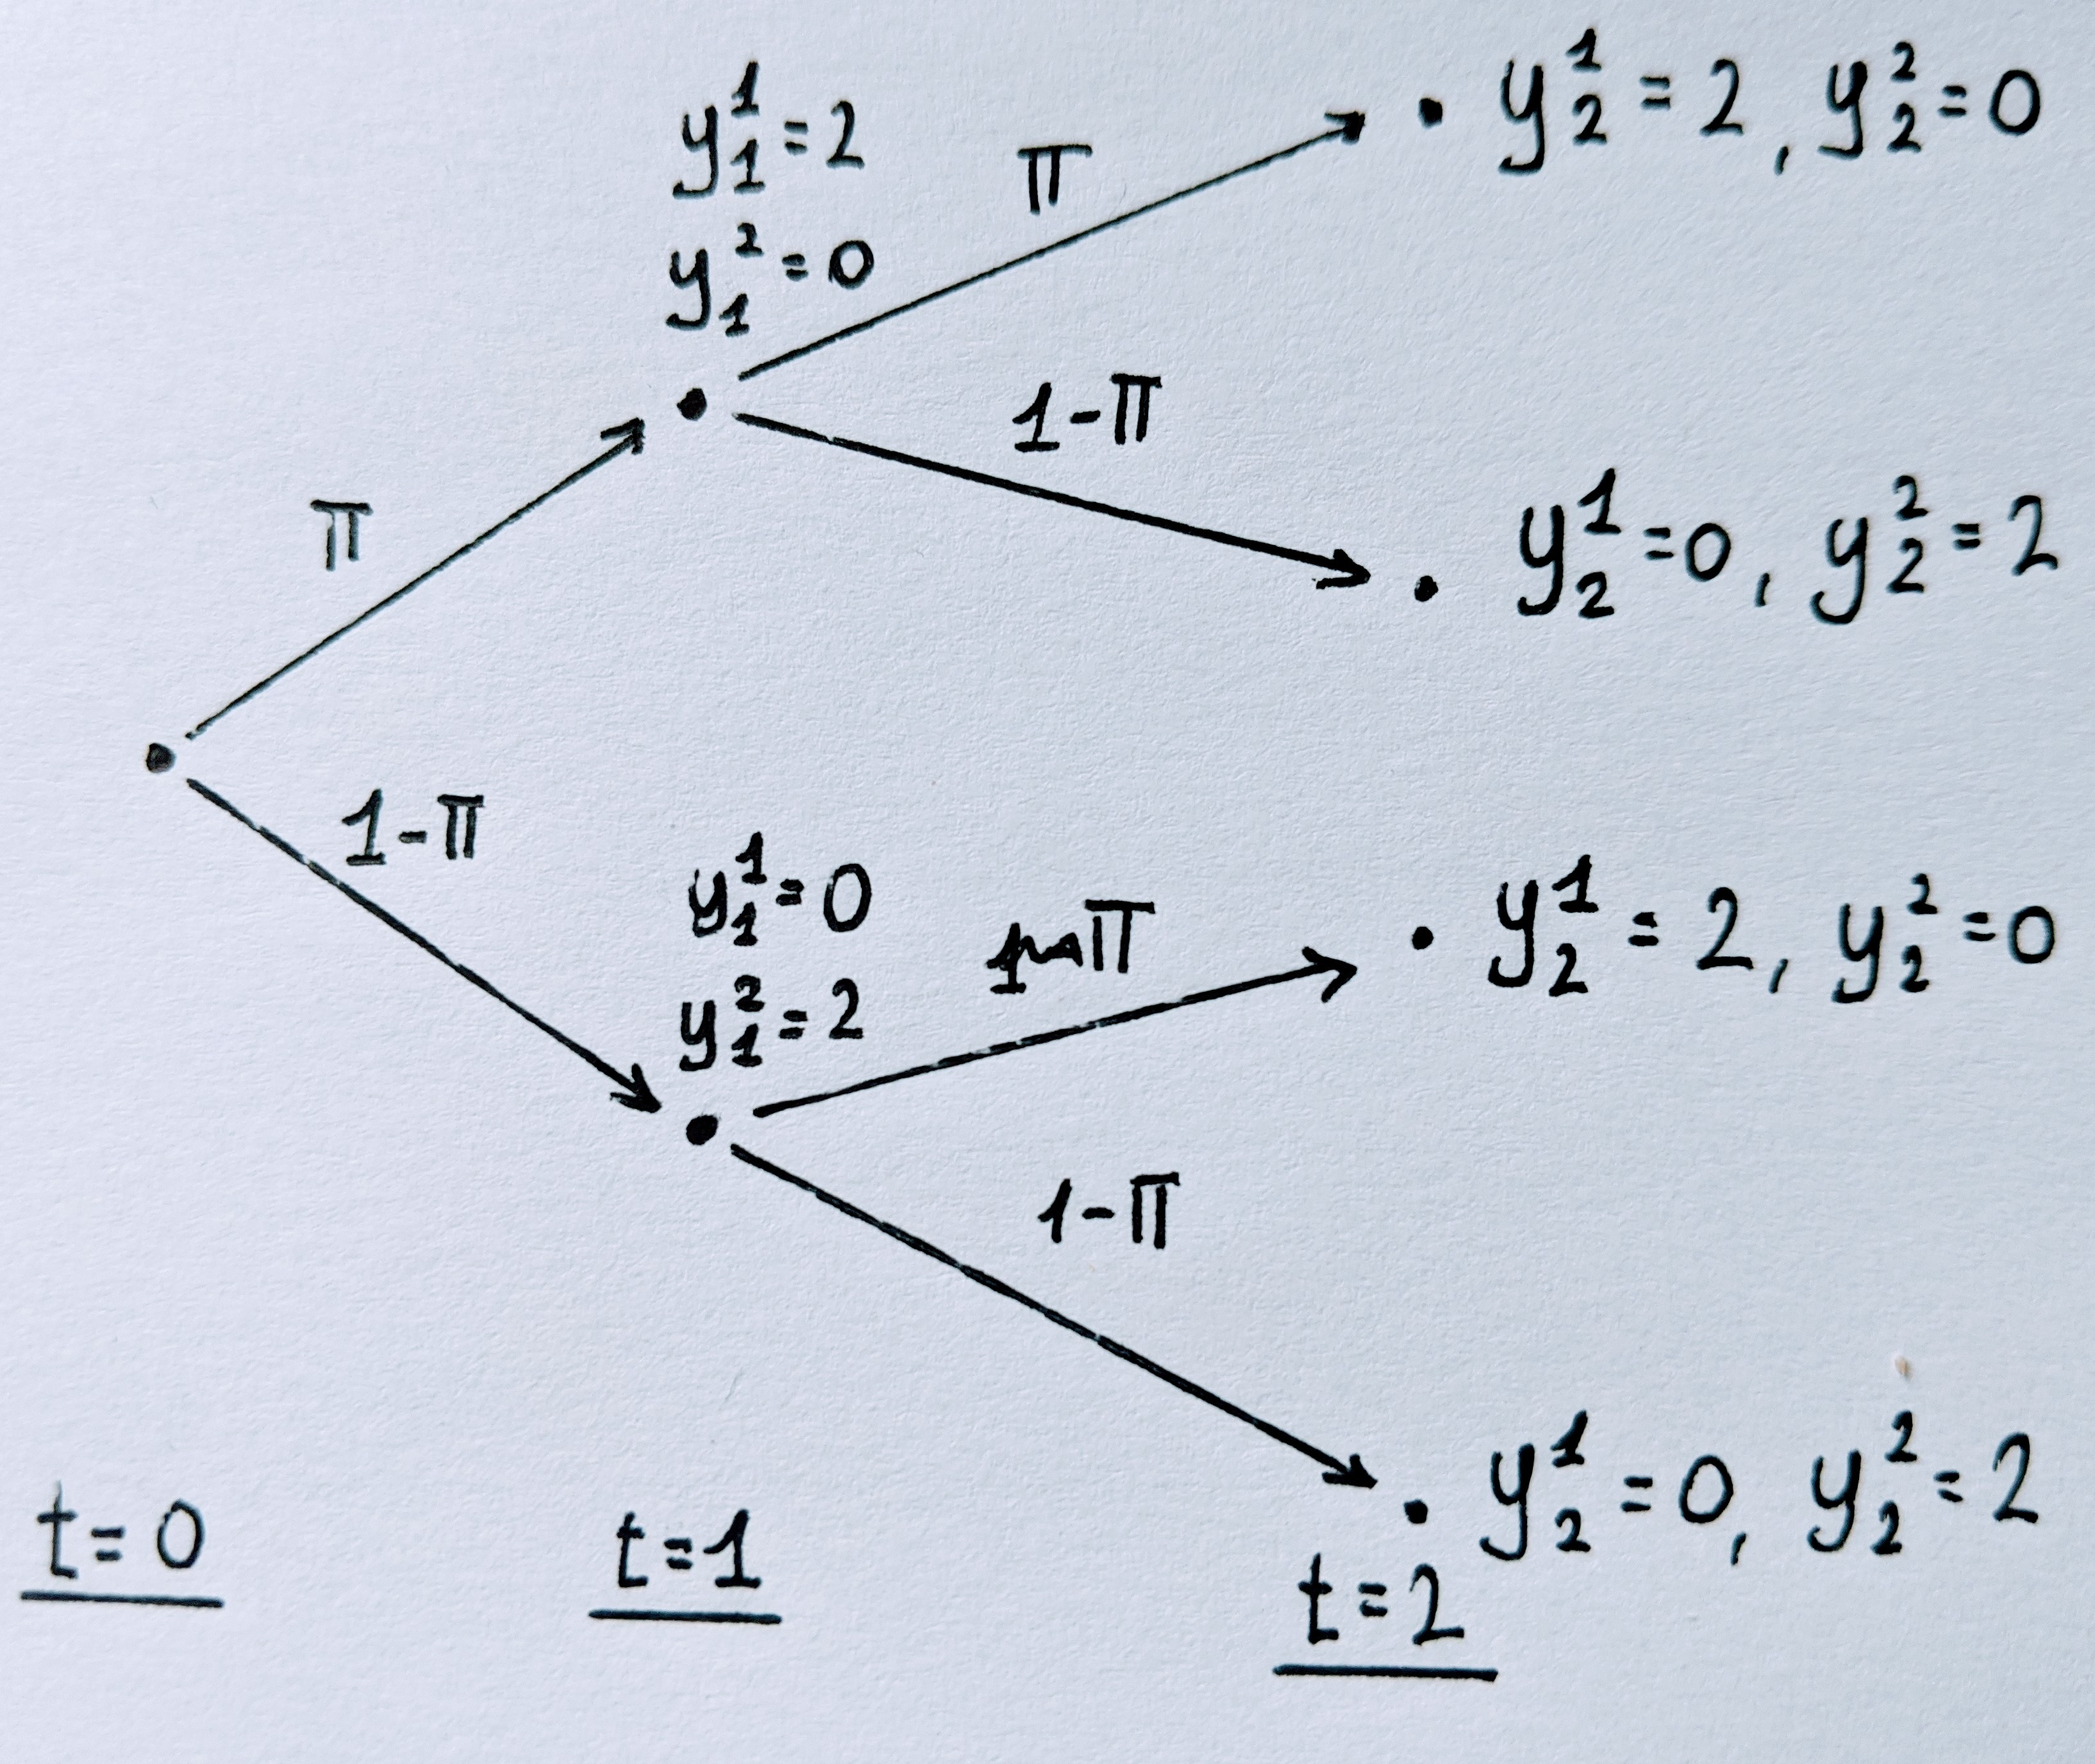
\includegraphics[width=0.5\linewidth]{./graph/Event_tree.jpg}
  \end{figure}

\item The new planners's maximization problem is:

  \begin{align*}
    & \max_{\{ c_t^1, c_t^2 \}^{2}_{t = 1}} \sum^2_{t=0} \sum_{s^t} \beta^t \pi(s^t) [\alpha \ln c_t^1(s^t) + (1-\alpha) \ln c_t^2(s^t)] \\
    & \text{s.t.} \\
    & c_t^i(s^t) \geq 0 \qquad \forall i, t \\
    & c^1_t(s^t) + c^2_t(s^t) = y_t^1(s^t) +  y_t^2(s^t)\quad \forall t.
  \end{align*}

  Notice that the resource constraint is such that

    $$
      c^1_t(s^t) + c^2_t(s^t) = y_t^1(s^t) +  y_t^2(s^t) = [\pi \cdot 2 + (1-\pi) \cdot 0] + [(1-\pi) \cdot 2 + \pi \cdot 0] = 2 \qquad \forall s^t, \forall t \in (1,2),
    $$

  that is, the amount of resources available to the planner in each period is equal to 2 with probability 1. Therefore the planner problem - and thus optimal consumption level - is not affected by past (or future) history nor by the probability of each state. The problem is thus exactly as before. Repeating the same passages  yields.

    \begin{align*}
      & c_t^1 (\alpha) = 2 \alpha \\
      & c_t^2 (\alpha) = 2(1-\alpha).
    \end{align*}

  \item The Lagrangian of the previous exercise is

    $$
      \mathbb{L} = \sum^2_{t=0} \sum_{s^t} \beta^t \pi(s^t) \left[ \alpha \ln c_t^1(s^t) + (1-\alpha) \ln c_t^2(s^t) + \frac{\mu_t}{2} \left(2 - c^1_t(s^t) - c_t^2(s^t) \right)\right].
    $$

  The first order conditions for a generic $t \in (1, 2)$ that is, for $c_t^1(s^t)$ and $c_t^1(s^t)$ are:

  \begin{align*}
    & \frac{\alpha\beta^t \pi(s^t)}{c_t^1(s^t)} = \frac{\mu_t}{2} \\
    & \frac{(1 -\alpha)\beta^t \pi(s^t)}{c_t^1(s^t)} = \frac{\mu_t}{2}.
  \end{align*}

  Substituting the optimal consumption yield

  $$
    \frac{\mu_t}{2} = \frac{\alpha\beta^t \pi(s^t)}{ 2 \alpha} \quad \Rightarrow \quad \mu_t(s^t) = \beta^t \pi(s^t)
  $$

  $QED$

  The value for each $t$ and $s^t$ is:
  \begin{align*}
    & \mu_0(\pi)  = 1 \\
    & \mu_1(\pi)  = \beta \pi \\
    & \mu_1(1 - \pi)  = \beta (1 - \pi) \\
    & \mu_2(\pi, \pi)  = (\beta \pi)^2 \\
    & \mu_2(\pi, 1 - \pi)  = \beta^2 \pi (1 - \pi) \\
    & \mu_2(1 - \pi, \pi)  = \beta^2 \pi (1 - \pi) \\
    & \mu_2(1 - \pi, 1 - \pi)  = \beta^2 (1 - \pi)^2 \\
  \end{align*}

  \item As before, the transfer function is

    $$
      t^i(\alpha) = \sum_{t} \sum_{s^t} \mu_t(s^t) \left( c_t^i(\alpha)- y_t^i \right),
    $$

  that is

    $$
    t^1(\alpha) = (2\alpha - 1) + 2\beta \pi(\alpha - 1) + 2\beta (1 - \pi)\alpha + 2(\beta \pi)^2 (\alpha - 1) + 2 \beta^2 \pi (1 - \pi) (2 \alpha - 1) + 2 \beta^2 (1 - \pi)^2 \alpha.
    $$

  Setting  $t^1(\alpha)=0$ yields
  $$
  (2\alpha - 1) + 2\beta \pi(\alpha - 1) + 2\beta (1 - \pi)\alpha + 2(\beta \pi)^2 (\alpha - 1) + 2 \beta^2 \pi (1 - \pi) (2 \alpha - 1) + 2 \beta^2 (1 - \pi)^2 \alpha = 0.
  $$

  That is:

  \begin{align*}
    2 \alpha & = \frac{1 + 2\beta\pi + 2 (\beta\pi)^2 + 2\beta^2\pi(1-\pi)}{1 + \beta\pi + \beta(1 - \pi) + (\beta\pi)^2 + 2 \beta^2\pi(1-\pi) + \beta^2 (1 - \pi)^2} \\
    & = \frac{1 + 2\beta\pi + 2\beta^2\pi }{1 + \beta + \beta^2\pi^2 + 2\beta^2 \pi + \beta^2(1-2\pi-\pi^2)} \\
    & = \frac{1 + 2\pi(\beta + \beta^2)}{1 + \beta + \beta^2}
  \end{align*}

  and

  \begin{align*}
    2(1-\alpha) & = 2 - 2\alpha = 2 -\frac{1 + 2\pi(\beta + \beta^2)}{1 + \beta + \beta^2} \\
    & = \frac{2 + 2\beta + 2 \beta^2 - 1 - 2\pi(\beta + \beta^2)}{1 + \beta + \beta^2} \\
    & = \frac{1 + 2(1 -\pi)(\beta + \beta^2)}{1 + \beta + \beta^2}
  \end{align*}

  $QED$.

  \item Since in a competitive equilibrium agents can consume only what they can afford, the planner's $\alpha$ that sustain such an equilibrium must represent the differences in the discounted expected stream of incomes between the two player. If $\pi = 0.5$ then the agents have the same expected income for each period. Therefore their expected income stream is the same, no matter the discount factor.

  \item If $\pi > 0.5$, then agent 1 is endowed, in expectation, with a larger income compared with player 2. Therefore he will be able to consume more than the other agent $\Leftrightarrow$ a pareto equilibrium with weight $\alpha > 0.5$.

\item Solving for sequential market equilibrium price:

Intertemporal budget constraint: 
\begin{equation*}
    c_{t}^{i}(s^t)+\sum_{s_{t+1}}a_{t+1}^{i}(s_{t+1},s^{t})q_t(s_{t+1}|s^{t})\leq y_{t}^{i}(s^t)+a_{t}^{i}(s^t)
\end{equation*}
No-Ponzi condition: 
\begin{equation*}
    -a_{t+1}^{i}(s^{t+1}) \leq A_{t+1}^{i}(s^{t+1})
\end{equation*}
The Lagrangian for the consumer problem will be given by: 


\begin{multline*}
    \mathcal{L}=\sum_{t=0}^{\infty}\sum_{s^t}\bigg\{
    \beta^t u(c_{t}^{i}(s^t))\pi_t(s^t)+\eta_{t}^{i}(s^t)\bigg[y_{t}^{i}(s^t)+a_{t}^{i}(s^t)-c_{t}^{i}(s^t)-\sum_{s^{t+1}}a_{t}^{i}(s_{t+1},s^t)q_t(s_{t+1}|s^{t})\bigg]\\
    +\sum_{s^{t+1}}\nu_{t}^{i}(s_{t+1},s^t)\bigg[A_{t+1}^{i}(s^{t+1})+a_{t+1}^{i}(s^{t+1})\bigg]\bigg\}
\end{multline*}
for a given initial wealth $a_0^{i}(s_0)$\\

First order conditions w.r.t. $c_{t}^{i}(s^t)$ and $a_{t}^{i}(s_{t+1},s^t)$:
\begin{equation*}
    \beta^t u'(c_{t}^{i}(s^t))\pi_t(s^t)-\eta_{t}^{i}(s^t)=0
\end{equation*}
\begin{equation*}
    -\eta_{t}^{i}(s^t)q_t(s_{t+1}|s^{t})+\nu_{t}^{i}(s_{t+1},s^t)+\eta_{t}^{i}(s_{t+1},s^t)=0
\end{equation*}
Because of the Inada conditions, the debt limit constraint will not be binding at the optimum.

\begin{center}
\Longrightarrow $\nu_{t}^{i}(s_{t+1},s^t)=0$, \forall t, s^t, s_{t+1}\Longrightarrow\hspace{1mm} $-\eta_{t}^{i}(s^t)q_t(s_{t+1}|s^{t})+\eta_{t}^{i}(s_{t+1},s^t)=0$
\end{center}
We have
\begin{equation*}
        \beta^t u'(c_{t}^{i}(s^t))\pi_t(s^t)-\eta_{t}^{i}(s^t)=0
\end{equation*}
\begin{equation*}
    -\eta_{t}^{i}(s^t)q_t(s_{t+1}|s^{t})+\eta_{t}^{i}(s_{t+1},s^t)=0
\end{equation*}
Substituting first equation in the second yields:
\begin{equation}
    q_t(s_{t+1}|s^{t})=\beta\frac{u'(c_{t+1}^{i}(s^{t+1}))}{u'(c_{t}^{i}(s^t))}\pi_t(s_{t+1}|s^{t}) \hspace{5mm} \forall t, s^t, s_{t+1}
\end{equation}

Notice that from F.O.C for Arrow-Debreu market, for agent $i$, we have that 
\begin{equation*}
     \beta^t u'(c_{t}^{i}(s^t))\pi_t(s^t)=\mu_i p_t(s^t)
\end{equation*}
\begin{equation*}
     \beta^{t+1} u'(c_{t+1}^{i}(s^{t+1}))\pi_t(s^{t+1})=\mu_i p_{t+1}(s^{t+1})
\end{equation*}
Dividing the second equation by the first:
\begin{equation}
    \frac{p_{t+1}(s^{t+1})}{p_t(s^t)}=\beta\frac{u'(c_{t+1}^{i}(s^{t+1}))}{u'(c_{t}^{i}(s^t))}\pi_t(s_{t+1}|s^{t}) \hspace{5mm} \forall t, s^t, s_{t+1}
\end{equation}
From (1) and (2):
\begin{equation*}
   q_t(s_{t+1}|s^{t}) =\frac{p_{t+1}(s^{t+1})}{p_t(s^t)} \hspace{5mm} (q.e.d)
\end{equation*}

\item Using the result

  $$
    \mu_t(s^t) = p_t(s^t) = \beta^t \pi(s^t),
  $$

  it follows that

  \begin{align*}
    & q_1(s^1) = \mu_1(s^1) \\
    & q_1(s^1,s^2) = \frac{\mu_1(s^2)}{\mu_1(s^1)}.
  \end{align*}

  Therefore

  \begin{align*}
    & q_1(\pi) = \beta \pi \\
    & q_1(1 - \pi) = \beta (1 - \pi) \\
    & q_2(\pi, \pi) = \frac{(\beta\pi)^2}{\beta \pi} = \beta \pi \\
    & q_2(1 - \pi, \pi) = \frac{\beta^2\pi(1-\pi)}{\beta (1 - \pi)} = \beta \pi \\
    & q_2(\pi, 1 - \pi) = \frac{\beta^2\pi(1-\pi)}{\beta \pi} = \beta ( 1 - \pi) \\
    & q_2(1 - \pi, 1 - \pi) = \frac{\beta^2(1-\pi)^2}{\beta (1 - \pi)} = \beta (1 - \pi).
  \end{align*}

\end{itemize}

The intuition for these prices is that they ensure the no arbitrage condition. For example, in period 0 you can buy one unit of consumption delivered in $t+1$ at price $p_{t+1}$. Then sell this unit in period $t$ to earn $q_{t}$ units of consumption delivered in period $t$. Hence, in period 0, you can sell $q_t$ units of consumption delivered in t at price $p_t$, earn $p_{t}q_{t}$ in period 0. By no arbitrage (and noting that the income process has no memory):
\begin{equation*}
    -p_{t+1}+p_tq_t=0 \hspace{5mm}(Q.E.D)
\end{equation*}
\end{document}
